\documentclass[11pt]{amsart}

\usepackage[T1]{fontenc}
\usepackage[utf8]{inputenc}
\usepackage{lmodern}
\usepackage{amsmath,amssymb,amsfonts,amsthm,mathtools}
\usepackage{geometry}
\usepackage{graphicx}
\usepackage[hidelinks]{hyperref}

\geometry{margin=1in}
\numberwithin{equation}{section}
\setcounter{tocdepth}{3}
\setcounter{secnumdepth}{3}

\theoremstyle{plain}
\newtheorem{theorem}{Theorem}[section]
\newtheorem{proposition}[theorem]{Proposition}
\newtheorem{lemma}[theorem]{Lemma}
\newtheorem{corollary}[theorem]{Corollary}

\theoremstyle{definition}
\newtheorem{definition}[theorem]{Definition}

\theoremstyle{remark}
\newtheorem{remark}[theorem]{Remark}

\title{Deterministic Phase Criteria for the Four-Step Pearson--Kluyver Law}
\author{Victor Casana}
\date{June 28, 2026}
\subjclass[2020]{11L03, 11K06, 60F05, 60G50}
\keywords{uniform distribution, Weyl criterion, van der Corput estimates, random walks, Pearson--Kluyver density}

\begin{document}
\begin{abstract}
We prove deterministic phase criteria under which the difference of two oriented chords has the four-step Pearson--Kluyver radial law. The central point is that a deterministic two-chord observable can have the same radial limit as four independent random unit steps. For
\(
\Delta_{h,g}(k)=(z_{k+h}-z_k)-(w_{k+g}-w_k),
\)
with fixed independent lags \(h\) and \(g\), this happens when the four-phase vector
\((\theta_{k+h},\theta_k,\phi_{k+g},\phi_k)\) is equidistributed in \(\mathbb T^4\). The limit is therefore not tied to the nearest-neighbour lag \(h=1\), not tied to the diagonal constraint \(h=g\), and not produced by a single chord. The paper gives a Weyl--van der Corput criterion, stated in terms of integer phase combinations and derivatives, and records explicit analytic pass/fail classes including power-log phases, affine chord collapse, logarithmic phases, log-log phases, and convergent phases.
\end{abstract}

\maketitle
\tableofcontents

\section{Introduction}
\label{sec:introduction}
The main object is the deterministic four-phase residual
\begin{equation}
\Delta_k=
\bigl(e^{if_1(k)}-e^{if_2(k)}\bigr)
-
\bigl(e^{if_3(k)}-e^{if_4(k)}\bigr),
\qquad k\in\mathbb Z_{\geq1}.
\label{eq:delta_general}
\end{equation}
We ask for checkable analytic conditions on the phase functions \(f_j\) which imply that \(|\Delta_k|\) converges in distribution to the radius of a four-step planar uniform random walk.

If \(U_1,\ldots,U_4\) are independent uniform variables on \([0,2\pi)\), set
\begin{equation}
R_4=\left|e^{iU_1}+e^{iU_2}+e^{iU_3}+e^{iU_4}\right|.
\label{eq:R4}
\end{equation}
Its density is the four-step Pearson--Kluyver density
\begin{equation}
p_4(r)=r\int_0^\infty J_0(rt)J_0(t)^4t\,dt,
\qquad 0<r<4,
\label{eq:p4}
\end{equation}
as treated in the modern short-walk literature \cite{BorweinEtAl2012,BorweinStraubWan2013,Zhou2019}.

The question addressed here is different: when does a deterministic two-chord sequence land on that four-step law? The four-step law appears after subtracting two oriented chords and after the associated four phase coordinates become equidistributed. Weyl's criterion and van der Corput estimates provide the analytic bridge from phase growth to this four-phase Haar limit \cite{Weyl1916,VanDerCorput1923,GrahamKolesnik1991}.

\section{Finite Numerical Diagnostics}
\label{sec:numerical_diagnostics}
Before the analytic proof, we record the finite diagnostics which motivate the criterion. They are numerical evidence and controls for the mechanism, not proofs of a limiting theorem.

\begin{figure}[htbp]
\centering
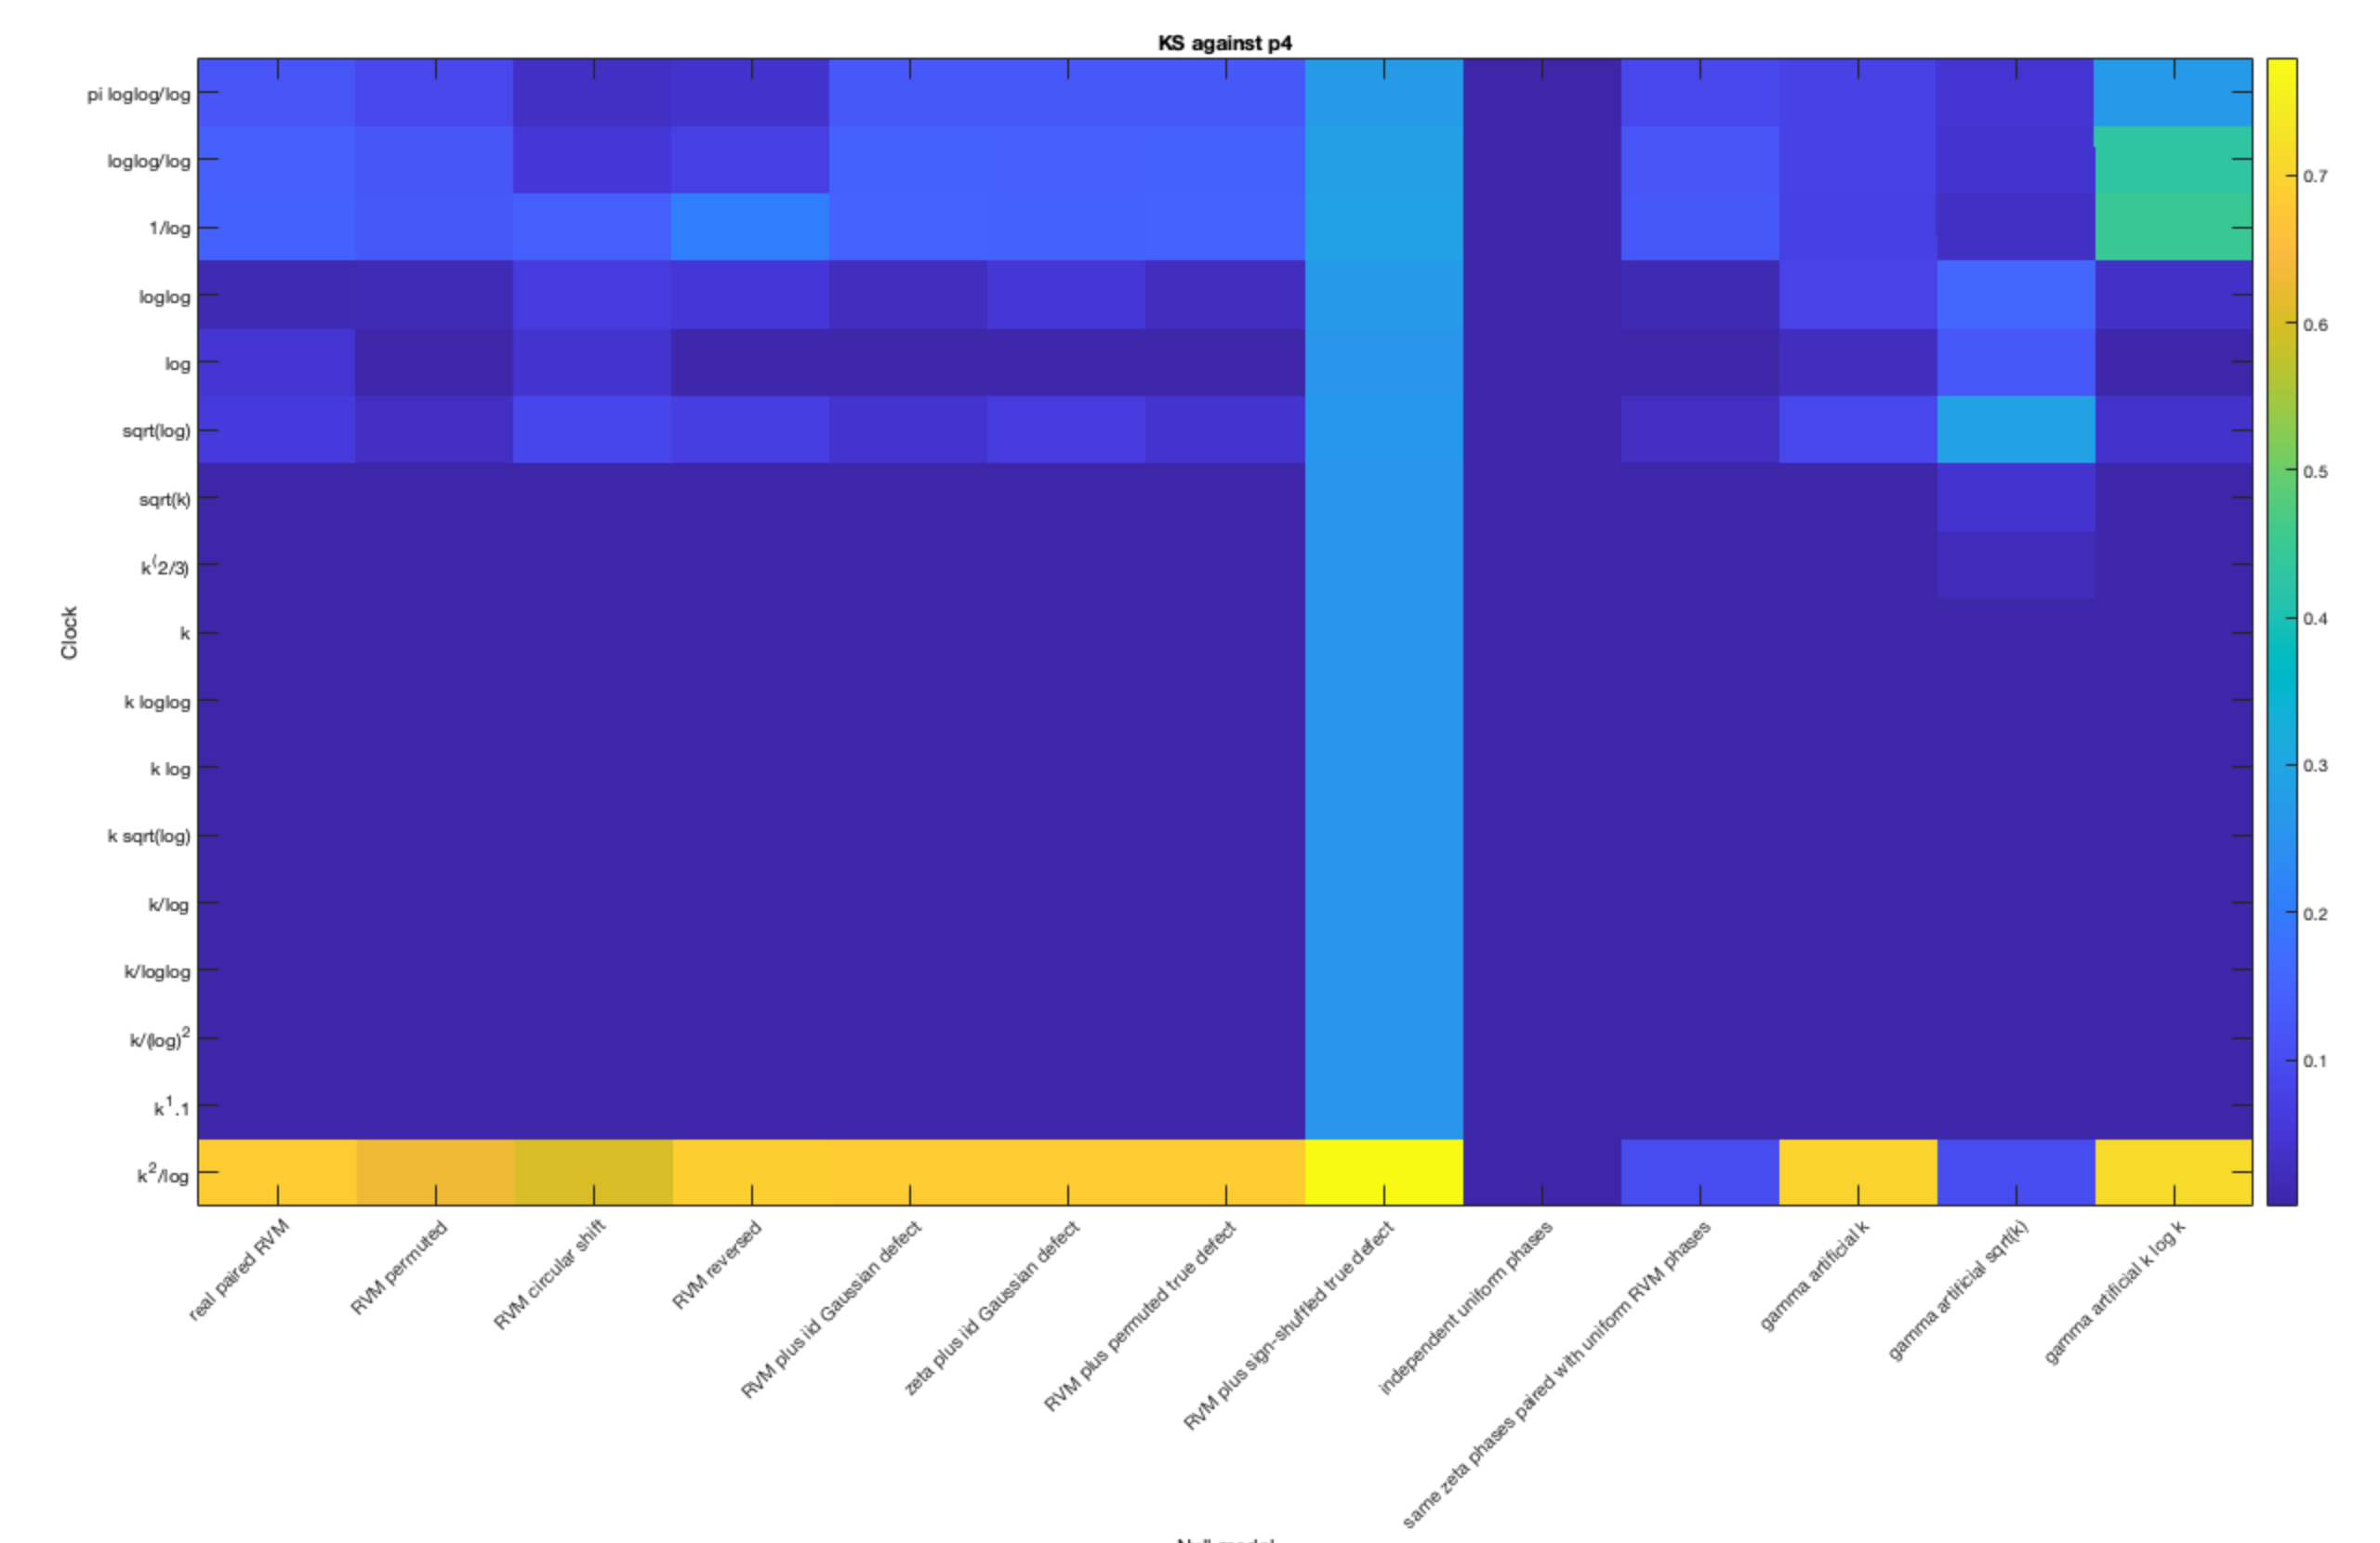
\includegraphics[width=\textwidth]{clock_model_ks_scan.png}
\caption{Finite KS scan against the normalized four-step Pearson--Kluyver law over clocks and phase models. This map is a clock/model diagnostic for the two-chord mechanism, separate from the RVM/zero data experiment.}
\label{fig:clock_model_scan}
\end{figure}

Figure \ref{fig:residual_controls} gives complementary histogram evidence. The left panels show several two-chord residual examples whose normalized radial histograms match the \(p_4\) profile at the tested scale. The right panels show the crucial control: the individual chords have large KS distance from \(p_4\), whereas their oriented difference has the Pearson--Kluyver profile.

\begin{figure}[htbp]
\centering
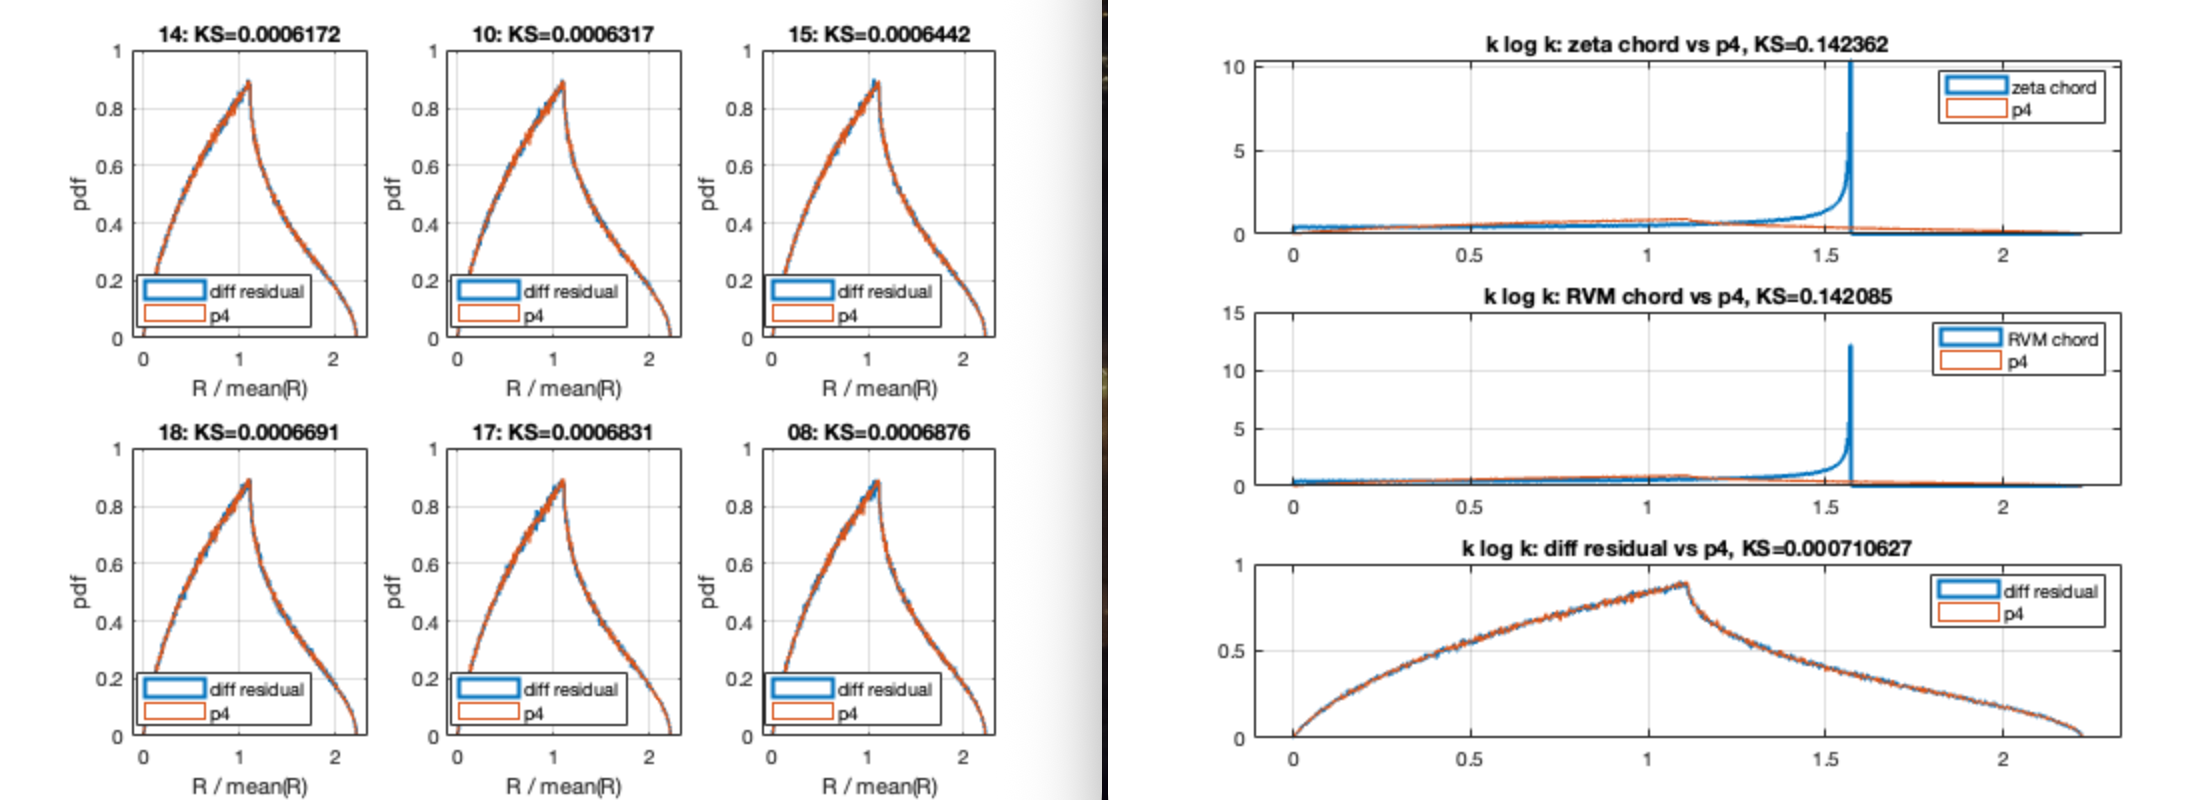
\includegraphics[width=\textwidth]{residual_single_chord_controls.png}
\caption{Residual examples and single-chord controls. The two-chord residuals match the \(p_4\) profile at the finite scale of the experiment; the individual chords do not.}
\label{fig:residual_controls}
\end{figure}

We also record a finite diagnostic on the paired RVM/zero data used in the computations. The files \texttt{zeross.bin} and \texttt{zLamb.bin} contain \(2{,}001{,}052\) paired ordinates; after the convention \(k\geq3\), the active phase sequence has \(2{,}001{,}050\) entries. With \(q_k=k\log k\), set
\begin{equation}
z_k=\exp(i\gamma_kq_k),
\qquad
w_k=\exp(i\lambda_kq_k),
\label{eq:rvm_zero_phases}
\end{equation}
and test
\begin{equation}
\Delta_{h,g}(k)=(z_{k+h}-z_k)-(w_{k+g}-w_k).
\label{eq:two_lag_residual}
\end{equation}
Across the tested two-lag matrix, the binned KS values against a simulated normalized four-step Pearson--Kluyver reference satisfy
\begin{equation}
0.00037577\leq D_{h,g}\leq0.00123132,
\qquad
\operatorname{median}D_{h,g}=0.000648068.
\label{eq:ks_range}
\end{equation}

\begin{figure}[htbp]
\centering
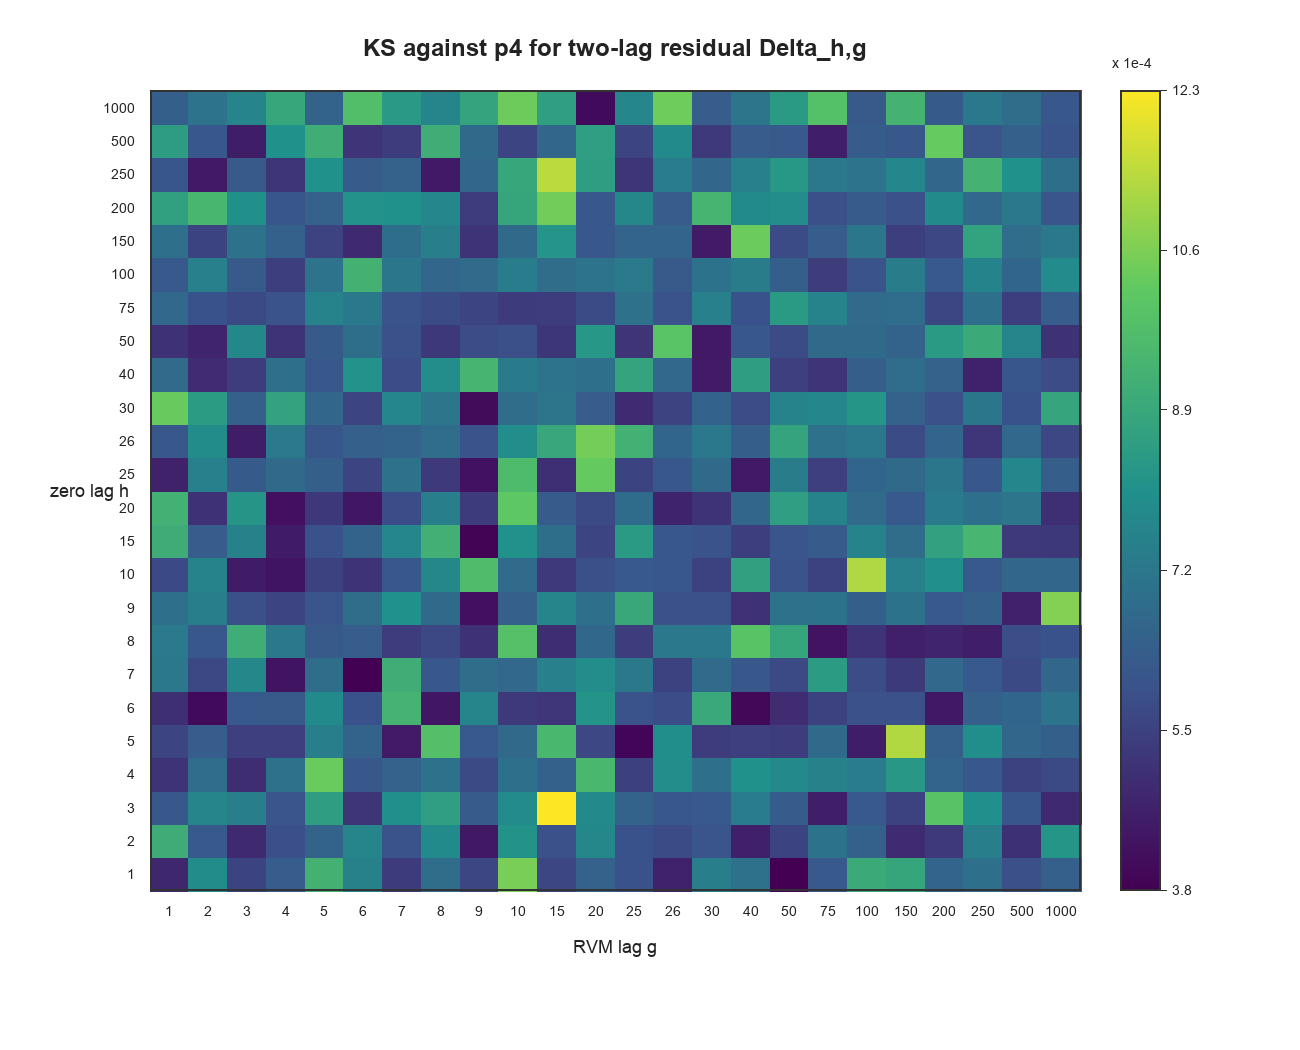
\includegraphics[width=0.86\textwidth]{rvm_zero_two_lag_ks.png}
\caption{Two-lag binned KS matrix for the normalized RVM/zero two-chord observable against the normalized four-step Pearson--Kluyver reference.}
\label{fig:rvm_zero_matrix}
\end{figure}

\section{The Four-Step Law and the Geometric Chord Integral}
\label{sec:four_step_law}

\begin{lemma}[Two-chord representation]
\label{lem:two_chord_representation}
Let
\begin{equation}
A=e^{i\alpha_2}-e^{i\alpha_1},
\qquad
B=e^{i\beta_2}-e^{i\beta_1},
\label{eq:A_B_chords}
\end{equation}
where \(\alpha_1,\alpha_2,\beta_1,\beta_2\) are independent and uniform on \([0,2\pi)\). Then \(|A-B|\) has the same distribution as \(R_4\).
\end{lemma}
\begin{proof}
The identity
\begin{equation}
A-B=e^{i\alpha_2}+e^{i(\alpha_1+\pi)}+e^{i(\beta_2+\pi)}+e^{i\beta_1}
\label{eq:four_step_identity}
\end{equation}
rewrites the difference of two chords as a sum of four unit vectors. Adding \(\pi\) preserves uniform measure on the circle and independence is preserved.
\end{proof}

\begin{proposition}[Geometric two-chord integral]
\label{prop:geometric_integral}
Let \(R=|A-B|\), with \(A,B\) as in \eqref{eq:A_B_chords}. For \(0<r<4\), the density of \(R\) is
\begin{equation}
p_R(r)=\frac{8r}{\pi^3}\int_0^2\!\int_0^2
\frac{\mathbf 1_{\{|a-b|<r<a+b\}}}
{\sqrt{(4-a^2)(4-b^2)((a+b)^2-r^2)(r^2-(a-b)^2)}}\,db\,da.
\label{eq:geometric_integral}
\end{equation}
Consequently \(p_R(r)=p_4(r)\) on \((0,4)\).
\end{proposition}
\begin{proof}
Put
\begin{equation}
a=|A|,
\qquad b=|B|,
\qquad \varphi=\angle(A,B)\in[0,\pi].
\label{eq:chord_coordinates}
\end{equation}
For one random chord,
\begin{equation}
a=2\left|\sin\frac{\alpha_2-\alpha_1}{2}\right|,
\label{eq:chord_length}
\end{equation}
and therefore
\begin{equation}
q(a)=\frac{2}{\pi\sqrt{4-a^2}},
\qquad 0<a<2.
\label{eq:chord_density}
\end{equation}
The two chord orientations are independent and isotropic, so \(\varphi\) is uniform on \([0,\pi]\), and
\begin{equation}
R^2=a^2+b^2-2ab\cos\varphi.
\label{eq:law_cosines}
\end{equation}
The equation \(R=r\) has a solution in \((0,\pi)\) precisely when \(|a-b|<r<a+b\). At this solution,
\begin{equation}
\sin\varphi_0=\frac{\sqrt{((a+b)^2-r^2)(r^2-(a-b)^2)}}{2ab}.
\label{eq:sin_phi0}
\end{equation}
The corresponding change of variables gives \eqref{eq:geometric_integral}. Lemma \ref{lem:two_chord_representation} then identifies the density with \(p_4\).
\end{proof}

\section{Deterministic Phase Residuals}
\label{sec:deterministic_residuals}

\begin{definition}[Four-phase sequence]
\label{def:four_phase_sequence}
Given real-valued phase functions \(f_1,\ldots,f_4\), define
\begin{equation}
\Phi_k=(f_1(k),f_2(k),f_3(k),f_4(k))\pmod{2\pi}\in\mathbb T^4.
\label{eq:Phi_k}
\end{equation}
\end{definition}

\begin{theorem}[Pushforward criterion]
\label{thm:pushforward}
If \(\Phi_k\) is equidistributed in \(\mathbb T^4\), then
\begin{equation}
|\Delta_k|\Rightarrow R_4.
\label{eq:pushforward_limit}
\end{equation}
\end{theorem}
\begin{proof}
The map
\begin{equation}
F(\theta_1,\theta_2,\theta_3,\theta_4)
=|e^{i\theta_1}-e^{i\theta_2}-e^{i\theta_3}+e^{i\theta_4}|
\label{eq:pushforward_map}
\end{equation}
is continuous on \(\mathbb T^4\). Equidistribution and the continuous mapping principle give the Haar pushforward, which is the law in Lemma \ref{lem:two_chord_representation}.
\end{proof}

\begin{definition}[Fixed-lag two-chord residual]
\label{def:fixed_lag_residual}
Let \(F,H\) be real-valued functions and let
\begin{equation}
\mathbf h=(h_1,h_2,h_3,h_4)\in\mathbb R^4,
\qquad h_1\neq h_2,
\qquad h_3\neq h_4.
\label{eq:lag_vector}
\end{equation}
Define
\begin{equation}
D_{k,\mathbf h}
=\bigl(e^{iF(k+h_1)}-e^{iF(k+h_2)}\bigr)
-\bigl(e^{iH(k+h_3)}-e^{iH(k+h_4)}\bigr),
\label{eq:Dkh}
\end{equation}
with phase vector
\begin{equation}
\Psi_{k,\mathbf h}
=(F(k+h_1),F(k+h_2),H(k+h_3),H(k+h_4))\pmod{2\pi}.
\label{eq:Psi_kh}
\end{equation}
\end{definition}

\begin{theorem}[Fixed-lag pushforward criterion]
\label{thm:fixed_lag_pushforward}
If \(\Psi_{k,\mathbf h}\) is equidistributed in \(\mathbb T^4\), then
\begin{equation}
|D_{k,\mathbf h}|\Rightarrow R_4.
\label{eq:fixed_lag_limit}
\end{equation}
\end{theorem}

\begin{corollary}[Independent fixed lags]
\label{cor:independent_lags}
Let \(z_k=e^{i\theta_k}\), \(w_k=e^{i\phi_k}\), and let \(h,g\) be fixed positive lags. If
\begin{equation}
(\theta_{k+h},\theta_k,\phi_{k+g},\phi_k)\pmod{2\pi}
\label{eq:lagged_four_phase_vector}
\end{equation}
is equidistributed in \(\mathbb T^4\), then \(|\Delta_{h,g}(k)|\Rightarrow R_4\).
\end{corollary}

\begin{proposition}[Single chords do not have the four-step law]
\label{prop:single_chord}
A single random chord has length
\begin{equation}
|e^{iU}-e^{iV}|=2\left|\sin\frac{U-V}{2}\right|,
\label{eq:single_chord_length}
\end{equation}
which is supported on \([0,2]\), whereas \(R_4\) is supported on \([0,4]\). Hence the laws differ.
\end{proposition}

\section{Weyl and Van der Corput Criteria}
\label{sec:weyl_vdc}

\begin{theorem}[Weyl criterion for the four phases]
\label{thm:weyl_four_phases}
The sequence \(\Phi_k\) is equidistributed in \(\mathbb T^4\) if and only if, for every \(\mathbf m=(m_1,m_2,m_3,m_4)\in\mathbb Z^4\setminus\{0\}\),
\begin{equation}
\frac1N\sum_{k\leq N}
\exp\left(i\sum_{j=1}^4m_jf_j(k)\right)\longrightarrow0.
\label{eq:weyl_criterion}
\end{equation}
\end{theorem}

\begin{corollary}[Weyl criterion for fixed lags]
\label{cor:weyl_fixed_lags}
The vector \(\Psi_{k,\mathbf h}\) is equidistributed if and only if, for every nonzero \(\mathbf m\in\mathbb Z^4\),
\begin{equation}
\frac1N\sum_{k\leq N}e^{iG_{\mathbf m,\mathbf h}(k)}\longrightarrow0,
\label{eq:lagged_weyl}
\end{equation}
where
\begin{equation}
G_{\mathbf m,\mathbf h}(t)
=m_1F(t+h_1)+m_2F(t+h_2)+m_3H(t+h_3)+m_4H(t+h_4).
\label{eq:Gmh}
\end{equation}
\end{corollary}

\begin{proposition}[Fixed-lag cancellation]
\label{prop:fixed_lag_cancellation}
Assume \(F,H\in C^2([T_0,\infty))\). For the \(F\)-part,
\begin{align}
m_1F(t+h_1)+m_2F(t+h_2)
&=(m_1+m_2)F(t)
 +(m_1h_1+m_2h_2)F'(t)+E_F(t),
\label{eq:fixed_lag_expansion}\\
E_F(t)
&=O_{\mathbf m,\mathbf h}\left(\sup_{|u-t|\leq H_0}|F''(u)|\right),
\qquad H_0=1+\max_j|h_j|.
\label{eq:fixed_lag_error}
\end{align}
If \(m_1+m_2=0\), the leading term is \(m_1(h_1-h_2)F'(t)\). The analogous statement holds for \(H\).
\end{proposition}

\begin{lemma}[Second-derivative van der Corput estimate]
\label{lem:vdc_second_derivative}
Let \(G\in C^2([N,2N])\). Suppose that for some \(0<\lambda\leq1\) and \(C\geq1\),
\begin{equation}
\lambda\leq |G''(t)|\leq C\lambda,
\qquad N\leq t\leq2N.
\label{eq:vdc_hypothesis}
\end{equation}
Then every interval \(I\subset[N,2N]\) satisfies
\begin{equation}
\left|\sum_{k\in I\cap\mathbb Z}e^{iG(k)}\right|
\ll_C N\lambda^{1/2}+\lambda^{-1/2}.
\label{eq:vdc_bound}
\end{equation}
\end{lemma}

\begin{theorem}[Dyadic curvature criterion]
\label{thm:dyadic_curvature}
For \(\mathbf m\in\mathbb Z^4\setminus\{0\}\), define
\begin{equation}
G_{\mathbf m}(t)=\sum_{j=1}^4m_jf_j(t).
\label{eq:Gm}
\end{equation}
Assume that for every nonzero \(\mathbf m\) there are constants \(C_{\mathbf m}\geq1\) and positive \(\lambda_N(\mathbf m)\) such that on every sufficiently large dyadic block
\begin{equation}
\lambda_N(\mathbf m)\leq|G_{\mathbf m}''(t)|\leq C_{\mathbf m}\lambda_N(\mathbf m),
\label{eq:curvature_bounds}
\end{equation}
and
\begin{equation}
\lambda_N(\mathbf m)\to0,
\qquad N^2\lambda_N(\mathbf m)\to\infty.
\label{eq:curvature_limits}
\end{equation}
Then \(\Phi_k\) is equidistributed in \(\mathbb T^4\), and consequently \(|\Delta_k|\Rightarrow R_4\).
\end{theorem}

\section{Explicit Phase Classes}
\label{sec:explicit_phase_classes}

\begin{corollary}[Power-log principal terms]
\label{cor:power_log}
Assume that every nonzero integer phase has a twice differentiable principal term
\begin{equation}
G_{\mathbf m}(t)=c_{\mathbf m}t^\rho(\log t)^\beta(1+o(1)),
\qquad c_{\mathbf m}\neq0.
\label{eq:power_log_principal}
\end{equation}
If \(0<\rho<2\), \(\rho\neq1\), the curvature criterion applies. It also applies for \(\rho=1\), \(\beta\neq0\), and for \(\rho=2\), \(\beta<0\).
\end{corollary}

\begin{proposition}[Exact linear four-phase flows]
\label{prop:linear_flows}
Let \(f_j(t)=a_jt+b_j\). Then \(\Phi_k\) is equidistributed in \(\mathbb T^4\) if and only if
\begin{equation}
m_1a_1+m_2a_2+m_3a_3+m_4a_4\notin2\pi\mathbb Z
\label{eq:linear_nonresonance}
\end{equation}
for every nonzero \(\mathbf m\in\mathbb Z^4\).
\end{proposition}

\begin{proposition}[Affine phases do not generate random chords]
\label{prop:affine_chords}
Let \(F(t)=ct+d\) and \(h_1\neq h_2\). Then
\begin{equation}
e^{iF(k+h_1)}-e^{iF(k+h_2)}
=e^{i(ck+d)}\bigl(e^{ich_1}-e^{ich_2}\bigr),
\label{eq:affine_chord}
\end{equation}
so the chord has constant length and the lagged pair is not equidistributed in \(\mathbb T^2\).
\end{proposition}

\begin{proposition}[Chord collapse]
\label{prop:chord_collapse}
Let \(F\in C^1([T_0,\infty))\), let \(h_1\neq h_2\), and assume \(F'(t)\to0\). Then
\begin{equation}
e^{iF(k+h_1)}-e^{iF(k+h_2)}\longrightarrow0.
\label{eq:chord_collapse}
\end{equation}
Hence the lagged pair cannot be equidistributed in \(\mathbb T^2\).
\end{proposition}

\begin{proposition}[The logarithmic phase fails]
\label{prop:log_phase_fails}
For \(c\neq0\),
\begin{equation}
\frac1N\sum_{k\leq N}e^{ic\log k}
=\frac{N^{ic}}{1+ic}+o(1),
\label{eq:log_phase_average}
\end{equation}
whose modulus stays bounded away from zero.
\end{proposition}

\begin{proposition}[The log-log phase fails]
\label{prop:loglog_phase_fails}
For \(c\neq0\),
\begin{equation}
\frac1N\sum_{3\leq k\leq N}e^{ic\log\log k}
=(\log N)^{ic}+O\left(\frac1{\log N}\right)+o(1),
\label{eq:loglog_phase_average}
\end{equation}
so the modulus tends to one.
\end{proposition}

\begin{proposition}[Convergent phases fail]
\label{prop:convergent_phases}
If for some nonzero integer test \(G_{\mathbf m}(k)\to\ell\pmod{2\pi}\), then
\begin{equation}
\frac1N\sum_{k\leq N}e^{iG_{\mathbf m}(k)}\longrightarrow e^{i\ell}.
\label{eq:convergent_phase_average}
\end{equation}
In particular, phases such as \(c/\log t\) fail for \(c\neq0\).
\end{proposition}

\section{Conclusion}
\label{sec:conclusion}
The deterministic mechanism is
\begin{equation}
\text{two deterministic oriented chords}
+\text{vanishing Weyl tests}
\Longrightarrow
\text{four-phase Haar limit}
\Longrightarrow
|\Delta_k|\Rightarrow R_4.
\label{eq:conclusion_mechanism}
\end{equation}
The random four-step law therefore enters through a deterministic two-chord mechanism: each single chord has the wrong radial law, but the difference of two oriented chords has the four-step law once the four endpoint phases equidistribute. The lags are fixed but independent; neither nearest-neighbour increments nor the diagonal condition \(h=g\) are part of the mechanism.

\begin{thebibliography}{99}
\bibitem{BorweinEtAl2012}
J.~M. Borwein, A. Straub, J. Wan, W. Zudilin, and D. Zagier,
\emph{Densities of short uniform random walks},
Canadian Journal of Mathematics \textbf{64} (2012), no.~5, 961--990.
DOI: 10.4153/CJM-2011-079-2; arXiv:1103.2995.

\bibitem{BorweinStraubWan2013}
J.~M. Borwein, A. Straub, and J. Wan,
\emph{Three-step and four-step random walk integrals},
Experimental Mathematics \textbf{22} (2013), no.~1, 1--14.
DOI: 10.1080/10586458.2013.748379.

\bibitem{Boshernitzan1994}
M. Boshernitzan,
\emph{Uniform distribution and Hardy fields},
Journal d'Analyse Mathématique \textbf{62} (1994), 225--240.
DOI: 10.1007/BF02835955.

\bibitem{GrahamKolesnik1991}
S.~W. Graham and G. Kolesnik,
\emph{Van der Corput's Method of Exponential Sums},
London Mathematical Society Lecture Note Series, vol.~126,
Cambridge University Press, 1991.
DOI: 10.1017/CBO9780511661976.

\bibitem{VanDerCorput1923}
J.~G. van der Corput,
\emph{Zahlentheoretische Abschätzungen mit Anwendung auf Gitterpunktprobleme},
Mathematische Zeitschrift \textbf{17} (1923), 250--259.
DOI: 10.1007/BF01504346.

\bibitem{Weyl1916}
H. Weyl,
\emph{Über die Gleichverteilung von Zahlen mod. Eins},
Mathematische Annalen \textbf{77} (1916), 313--352.
DOI: 10.1007/BF01475864.

\bibitem{Zhou2019}
Y. Zhou,
\emph{On Borwein's conjectures for planar uniform random walks},
Journal of the Australian Mathematical Society \textbf{107} (2019), no.~3, 392--411.
DOI: 10.1017/S1446788719000351; arXiv:1708.02857.
\end{thebibliography}

\end{document}
